\clearpage

\section{Physical Topology}\label{Reference_Network_Topology}
\begin{tcolorbox}	
\begin{tabular}{p{2.75cm} p{0.2cm} p{10.5cm}} 	
\textbf{Student Name}  &:& Tiago Esteves    (October 03, 2017 - )\\
\end{tabular}
\end{tcolorbox}
\vspace{11pt}

In the following figure we can see that our reference network consists of 6 nodes and 8 bidirectional links.
Besides this layout of links and nodes will also need to know the average length of the links.
This value varies depending on the length of each link so it will be necessary to define all distances between the respective nodes.
Finally, it is also necessary to indicate the total traffic used in this network so the ODU matrices will be created.\\

\begin{figure}[h!]
\centering
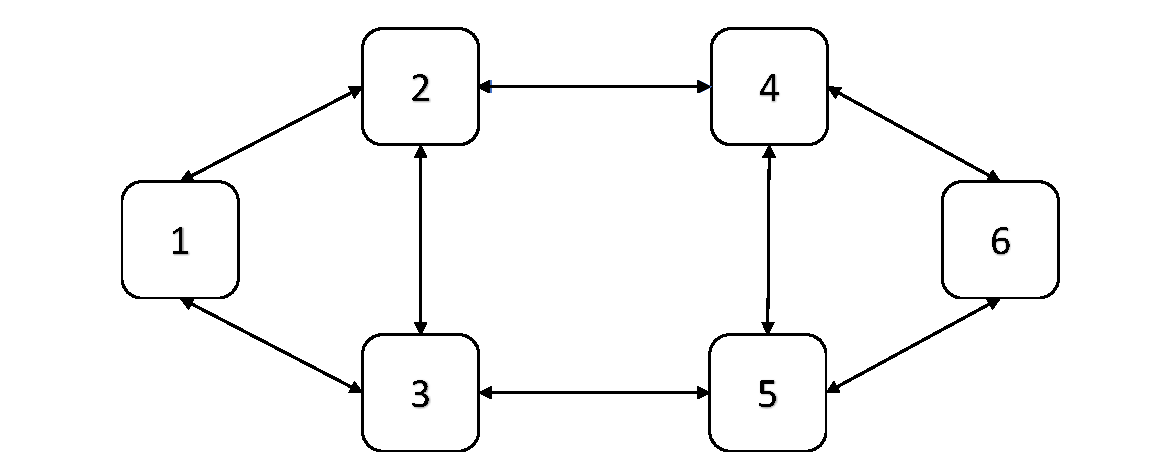
\includegraphics[width=\textwidth]{sdf/reference_network/figures/RedeTeste}
\caption{Physical topology of the reference network.}
\end{figure}

\vspace{11pt}
The distance matrix for this reference network is the same regardless of its associated traffic.
The values indicated in the distance matrix, referred to below, are expressed in kilometers (Km) and, as it could not be otherwise, this matrix is symmetric because the distance from $1$ to $2$ must be the same as $2$ to $1$.\\

\[
Dist=
  \begin{bmatrix}
    0 & 460 & 663 & 0 & 0 & 0 \\
    460 & 0 & 75 & 684 & 0 & 0 \\
    663 & 75 & 0 & 0 & 890 & 0 \\
    0 & 684 & 0 & 0 & 103 & 764 \\
    0 & 0 & 890 & 103 & 0 & 361 \\
    0 & 0 & 0 & 764 & 361 & 0
  \end{bmatrix}
\]

\newpage
For this project has to take into consideration the table \ref{table_ref_net} because in it we can see the values of the variables associated with this network.\\

\begin{table}[h!]
\centering
\begin{tabular}{|| c | c | c||}
 \hline
 Constant & Description & Value \\
 \hline\hline
 N & Number of nodes & 6 \\
 L & Number of bidirectional links & 8 \\
 <$\delta$> & Node out-degree & 2.667 \\
 <len> & Mean link length (km) & 500 \\
 <h> & Mean number of hops for working paths & 1.533 \\
 <h'> & Mean number of hops for backup paths & 2.467 \\
 \hline
\end{tabular}
\caption{Table of reference network values}
\label{table_ref_net}
\end{table}


\section{Traffic Matrices}\label{Reference_Network_Traffic}
\begin{tcolorbox}	
\begin{tabular}{p{2.75cm} p{0.2cm} p{10.5cm}} 	
\textbf{Student Name}  &:& Tiago Esteves    (October 03, 2017 - )\\
\end{tabular}
\end{tcolorbox}
\vspace{11pt}

For a better interpretation of the later results we will assume three traffic models for this network.
Being the first model with a low traffic scenario, the second with a medium traffic scenario and a last one with a high traffic scenario.
For each scenario it will be necessary to create different traffic matrices and to know the traffic of the network we will use five matrices of traffic.
These traffic matrices are represented by ODU0, ODU1, ODU2, ODU3 and ODU4 where each one has a certain bit rate.
The ODU0 corresponds to 1.25 Gbits/s, the ODU1 corresponds to 2.5 Gbits/s, the ODU2 corresponds to 10 Gbits/s, the ODU3 corresponds to 40 Gbits/s and finally the ODU4 corresponds to 100 Gbits/s.
As we can see below, these arrays are bi-directional because they are symmetric arrays and as such, the traffic sent in a certain direction must be the same traffic sent in that opposite direction.

\subsection{Low traffic scenario (0.5 Tbits/s)}\label{low_traffic_scenario}

The traffic matrices for this scenario are:

\[
ODU0=
  \begin{bmatrix}
    0 & 5 & 1 & 3 & 1 & 3 \\
    5 & 0 & 0 & 1 & 5 & 0 \\
    1 & 0 & 0 & 1 & 4 & 1 \\
    3 & 1 & 1 & 0 & 1 & 1 \\
    1 & 5 & 4 & 1 & 0 & 3 \\
    3 & 0 & 1 & 1 & 3 & 0
  \end{bmatrix}
\qquad ODU1=
  \begin{bmatrix}
    0 & 2 & 4 & 2 & 0 & 5 \\
    2 & 0 & 0 & 3 & 1 & 1 \\
    4 & 0 & 0 & 1 & 1 & 0 \\
    2 & 3 & 1 & 0 & 1 & 3 \\
    0 & 1 & 1 & 1 & 0 & 1 \\
    5 & 1 & 0 & 3 & 1 & 0
  \end{bmatrix}
\]
\[
ODU2=
  \begin{bmatrix}
    0 & 1 & 1 & 1 & 0 & 0 \\
    1 & 0 & 0 & 0 & 1 & 0 \\
    1 & 0 & 0 & 1 & 1 & 0 \\
    1 & 0 & 1 & 0 & 1 & 0 \\
    0 & 1 & 1 & 1 & 0 & 1 \\
    0 & 0 & 0 & 0 & 1 & 0
  \end{bmatrix}
\qquad ODU3=
  \begin{bmatrix}
    0 & 0 & 0 & 0 & 0 & 0 \\
    0 & 0 & 1 & 0 & 0 & 1 \\
    0 & 1 & 0 & 0 & 1 & 0 \\
    0 & 0 & 0 & 0 & 0 & 0 \\
    0 & 0 & 1 & 0 & 0 & 0 \\
    0 & 1 & 0 & 0 & 0 & 0
  \end{bmatrix}
\]
\[
ODU4=
  \begin{bmatrix}
    0 & 0 & 0 & 0 & 0 & 0 \\
    0 & 0 & 0 & 0 & 0 & 1 \\
    0 & 0 & 0 & 0 & 0 & 0 \\
    0 & 0 & 0 & 0 & 0 & 0 \\
    0 & 0 & 0 & 0 & 0 & 1 \\
    0 & 1 & 0 & 0 & 1 & 0
  \end{bmatrix}
\]

\vspace{17pt}
Through these ODU's we can calculate total network traffic for the low traffic scenario:\\

$T_1^0$ = 60x1.25 = 75 Gbits/s \qquad
$T_1^1$ = 50x2.5 = 125 Gbits/s \qquad
$T_1^2$ = 16x10 = 160 Gbits/s \\

$T_1^3$ = 6x40 = 240 Gbits/s \quad
$T_1^4$ = 4x100 = 400 Gbits/s \\

$T_{1}$ = 75 + 125 + 160 + 240 + 400 = 1000 Gbits/s \qquad
$T$ = 1000/2 = \textbf{0.5 Tbits/s}\\

Where the variable $T_1^x$ represents the unidirectional traffic of the ODUx, for example, $T_1^0$ represents the unidirectional traffic of the ODU0 and $T_1^1$ represents the unidirectional traffic of the ODU1. The variable $T_{1}$ represents the total of unidirectional traffic that is injected into the network and finally the variable $T$ represents the total of bidirectional traffic.\\

\subsection{Medium traffic scenario (5 Tbits/s)}\label{medium_traffic_scenario}

The traffic matrices for this scenario are:

\[
ODU0=
  \begin{bmatrix}
    0 & 50 & 10 & 30 & 10 & 30 \\
    50 & 0 & 0 & 10 & 50 & 0 \\
    10 & 0 & 0 & 10 & 40 & 10 \\
    30 & 10 & 10 & 0 & 10 & 10 \\
    10 & 50 & 40 & 10 & 0 & 30 \\
    30 & 0 & 10 & 10 & 30 & 0
  \end{bmatrix}
\quad ODU1=
  \begin{bmatrix}
    0 & 20 & 40 & 20 & 0 & 50 \\
    20 & 0 & 0 & 30 & 10 & 10 \\
    40 & 0 & 0 & 10 & 10 & 0 \\
    20 & 30 & 10 & 0 & 10 & 30 \\
    0 & 10 & 10 & 10 & 0 & 10 \\
    50 & 10 & 0 & 30 & 10 & 0
  \end{bmatrix}
\]
\[
ODU2=
  \begin{bmatrix}
    0 & 10 & 10 & 10 & 0 & 0 \\
    10 & 0 & 0 & 0 & 10 & 0 \\
    10 & 0 & 0 & 10 & 10 & 0 \\
    10 & 0 & 10 & 0 & 10 & 0 \\
    0 & 10 & 10 & 10 & 0 & 10 \\
    0 & 0 & 0 & 0 & 10 & 0
  \end{bmatrix}
\quad ODU3=
  \begin{bmatrix}
    0 & 0 & 0 & 0 & 0 & 0 \\
    0 & 0 & 10 & 0 & 0 & 10 \\
    0 & 10 & 0 & 0 & 10 & 0 \\
    0 & 0 & 0 & 0 & 0 & 0 \\
    0 & 0 & 10 & 0 & 0 & 0 \\
    0 & 10 & 0 & 0 & 0 & 0
  \end{bmatrix}
\]
\[
ODU4=
  \begin{bmatrix}
    0 & 0 & 0 & 0 & 0 & 0 \\
    0 & 0 & 0 & 0 & 0 & 10 \\
    0 & 0 & 0 & 0 & 0 & 0 \\
    0 & 0 & 0 & 0 & 0 & 0 \\
    0 & 0 & 0 & 0 & 0 & 10 \\
    0 & 10 & 0 & 0 & 10 & 0
  \end{bmatrix}
\]

\vspace{17pt}
Through these ODU's we can calculate total network traffic for the medium traffic scenario:\\

$T_1^0$ = 600x1.25 = 750 Gbits/s \quad
$T_1^1$ = 500x2.5 = 1205 Gbits/s \quad
$T_1^2$ = 160x10 = 1600 Gbits/s \\

$T_1^3$ = 60x40 = 2400 Gbits/s \quad
$T_1^4$ = 40x100 = 4000 Gbits/s \\

$T_{1}$ = 750 + 1250 + 1600 + 2400 + 4000 = 10000 Gbits/s \qquad
$T$ = 10000/2 = \textbf{5 Tbits/s}\\

\subsection{High traffic scenario (10 Tbits/s)}\label{high_traffic_scenario}

The traffic matrices for this scenario are:

\[
ODU0=
  \begin{bmatrix}
    0 & 100 & 20 & 60 & 20 & 60 \\
    100 & 0 & 0 & 20 & 100 & 0 \\
    20 & 0 & 0 & 20 & 80 & 20 \\
    60 & 20 & 20 & 0 & 20 & 20 \\
    20 & 100 & 80 & 20 & 0 & 60 \\
    60 & 0 & 20 & 20 & 60 & 0
  \end{bmatrix}
\quad ODU1=
  \begin{bmatrix}
    0 & 40 & 80 & 40 & 0 & 100 \\
    40 & 0 & 0 & 60 & 20 & 20 \\
    80 & 0 & 0 & 20 & 20 & 0 \\
    40 & 60 & 20 & 0 & 20 & 60 \\
    0 & 20 & 20 & 20 & 0 & 20 \\
    100 & 20 & 0 & 60 & 20 & 0
  \end{bmatrix}
\]
\[
ODU2=
  \begin{bmatrix}
    0 & 20 & 20 & 20 & 0 & 0 \\
    20 & 0 & 0 & 0 & 20 & 0 \\
    20 & 0 & 0 & 20 & 20 & 0 \\
    20 & 0 & 20 & 0 & 20 & 0 \\
    0 & 20 & 20 & 20 & 0 & 20 \\
    0 & 0 & 0 & 0 & 20 & 0
  \end{bmatrix}
\quad ODU3=
  \begin{bmatrix}
    0 & 0 & 0 & 0 & 0 & 0 \\
    0 & 0 & 20 & 0 & 0 & 20 \\
    0 & 20 & 0 & 0 & 20 & 0 \\
    0 & 0 & 0 & 0 & 0 & 0 \\
    0 & 0 & 20 & 0 & 0 & 0 \\
    0 & 20 & 0 & 0 & 0 & 0
  \end{bmatrix}
\]
\[
ODU4=
  \begin{bmatrix}
    0 & 0 & 0 & 0 & 0 & 0 \\
    0 & 0 & 0 & 0 & 0 & 20 \\
    0 & 0 & 0 & 0 & 0 & 0 \\
    0 & 0 & 0 & 0 & 0 & 0 \\
    0 & 0 & 0 & 0 & 0 & 20 \\
    0 & 20 & 0 & 0 & 20 & 0
  \end{bmatrix}
\]

\vspace{17pt}
Through these ODU's we can calculate total network traffic for the high traffic scenario:\\

$T_1^0$ = 1200x1.25 = 1500 Gbits/s \qquad
$T_1^1$ = 1000x2.5 = 2500 Gbits/s \\

$T_1^2$ = 320x10 = 3200 Gbits/s \qquad
$T_1^3$ = 120x40 = 4800 Gbits/s \\

$T_1^4$ = 80x100 = 8000 Gbits/s \\

$T_{1}$ = 1500 + 2500 + 3200 + 4800 + 8000 = 20000 Gbits/s \\

$T$ = 20000/2 = \textbf{10 Tbits/s}\\

